\chapter{Supervised Learning in Feed Forward Networks}\label{ch_supervised_ff}
\chapterauthor{Jeff Yoshimi}
	
Having introduced supervised learning in chapter \extref{ch_supervised}, in this chapter we consider several supervised learning algorithms for feedforward networks in depth, and consider their implications for cognitive science. First, an early form of supervised learning called the ``Least Mean Squares rule'' or ``LMS rule''. Second, backpropagation, which adds a powerful method of learning \emph{internal representations} in a neural network. Third, we briefly discuss deep learning networks, which take backprop and apply it to networks with many layers off processing units. Finally, we show how even though these networks were mainly developed in engineering contexts, they have been used in connectionism  and computational cognitive science  to study the  kinds of representations that humans develop to do things like recognize faces.

\section{Least Mean Squares Rule}\label{lms_rule}

We now consider our first supervised learning algorithm in detail: the \glossary{Least Mean Square}s rule or ``LMS'' or ``Delta rule'', which uses a form of gradient descent to minimize the error on a training set. It makes a nice contrast with Hebbian learning. We have seen that repeated application of the Hebb rule tends to force weights to go to their maximum or minimum values. LMS is more stable: as we will see, repeated application of LMS shifts weights and biases incrementally up and down until they settle in on just the right values.\footnote{This rule is also known as the ``Widrow-Hoff'' rule, or the ``Delta Rule.'' It is a descendent of Rosenblatt's perceptron learning rule (\cite{rosenblatt1960perceptron}; also see chapter \extref{ch_history}). Rosenblatt's rule computed error using the output of a node with a threshold activation function on classification tasks. Since both targets and outputs were either 0 or 1, this led to weight and bias updates that were ``jittery'' and sometimes unstable. Widrow and Hoff made a slight change to the rule, computing the error based on how far the target values were from the weighted input, which varied continuously. This made learning smoother and more reliable. It also allowed the rule to be used on a broader class of problems, including classification and regression problems. Widrow and Hoff built a device that used the rule called an ``Adaline''. The Delta rule can be shown to be equivalent to ordinary least squares regression, which is why the phrase ``least mean squares'' is used. Terminology  in this  area is not entirely consistent. For example, any network trained by LMS is often called a ``Perceptron''. }  

Note that LMS is an algorithm that only works with 2-layer networks. It cannot be directly applied to multi-layer networks. That is an important limitation that is overcome by backprop, as we will see.
% For linear networks, it does not matter how many layers they are, they are the same. 
% Any linearly separable problem can be solved with this algorithm. The perceptron convergence theorem.

LMS follows the template from section \extref{SupervisedFirstPass}:  begin with  random parameters (weights and biases), iterate through each of the input patterns, compute outputs (this is sometimes called a ``forward pass''), and compare these outputs with desired or target outputs. That is, compute a set of row errors and then an overall error. Then, the weights and biases are adjusted in a way that reduces overall error, using gradient descent.  Weights and biases are changed in such a way that overall error decreases. The next time the network sees the same input vectors again, it should produce outputs on each node that are closer to the desired values.
% Discuss in a footnote (here  or above) convex optimization and how there is always a global minimum.
% https://towardsdatascience.com/understanding-convexity-why-gradient-descent-works-for-linear-regression-aaf763308708

Intuitively, the algorithm works like this (for positive valued inputs). If the output is too high, the error is negative. For example, if I wanted 4 but got 5, row error is $4-5 = -1$. I have to make the weights and bias a little bit lower to make the output lower. On the other hand, if the output is too low, the error is positive. For example, if I wanted 5 but got 4, error is $5-4 = 1$. I have to make the weights and bias a little larger. (Notice that multiplying the weights by the row error would send us in the right direction, and that larger errors will lead to larger weight changes). If the output is just right, don't change anything. By incrementally changing the weights and biases in this way, the network slowly learns to produce the correct response to all inputs. Think of this as a kind of {\bf Goldilocks principle}: just as someone might keep heating and cooling porridge until it is just right, we increase and decrease parameters until overall error is just right.\footnote{A useful picture showing how this method leads to a decision boundary that correctly classifies all training examples is here: \url{https://commons.wikimedia.org/wiki/File:Perceptron_example.svg}.}
% We can also think of this as a process of repeatedly testing the network and correcting for false positives (the output is too high; a ``type 1'' error) and false negatives (the output is too low; a ``type 2'' error) until the error rate is as low as possible. This analysis really only makes sense for binary variables and thus classification tasks. But it's useful to mention, once qualified.
 
\subsection{The Algorithm}

Now we can formally define the LMS rule, and verify that it causes the weights to change a such a way that the sum of squared errors (SSE) gets lower over time.\footnote{We will not formally derive it, or state the algorithm in its full generality. However, the derivation is not too difficult: the key step involves taking the derivative of the error function with respect to a weight (how much is error changing as a function of that particular weight). A brief derivation is at \url{https://en.wikipedia.org/wiki/Delta_rule} and a more detailed discussion is at \url{http://uni-obuda.hu/users/fuller.robert/delta.pdf}.}

% It's like Hebb but instead of target node we have error on target node. 
When applying the rule, a change in a weight $w_{i,j}$ is equal to the product of a learning rate $\epsilon$, the activation of the input node to that weight, $a_i$, and the difference between a desired and actual activation ($t_j - a_j$) for that node:
\begin{eqnarray*}
\Delta w_{i,j}  =  \epsilon a_i (t_j - a_j)
\end{eqnarray*}
Since $(t_j - a_j)$ is row error  (with a small ``e''), the rule says that the change in a weight is equal to a learning rate times the activation of the input node for that weight, times the error. This should make some intuitive sense. As we saw above in the goldilocks discussion, for positive inputs weights should be changed in the direction of row error. The input scales things so they work for positive or negative inputs and so that changes are bigger for bigger inputs, and the learning rate allows us to control how quickly learning happens. 

LMS also changes the bias $b_j$ of an output node $j$ as follows: 
\begin{eqnarray*}
\Delta b_j  =  \epsilon (t_j - a_j)
\end{eqnarray*}
That is, the change in a bias for a node $j$ is just the learning rate times the error on output node $j$.\footnote{Note that this is really the same as the weight change rule, if we think of the bias in terms another input neuron, clamped at 1, and attached to this output neuron by a modifiable weight (which is in effect the bias).}

Applying the rule involves two stages at each iteration. First, a ``forward pass'', where we compute the output of the network for a given input pattern. Then a ``backward pass'' or ``weight update'' pass where we compute the error for each output node (how close was the node's output to the target value?) and then use this error to change its fan-in weights and its bias. Then we repeat the process for every output node on every input pattern, until we have worked our way through the whole training set. 

% Talk about how divergence looks in this kind of case. And add some practice examples that show it happening. E.g. Given a1 = -3, w12=4, t = 0, epsilon = 1, what is w12'?


\subsection{Example}\label{lms_example}

In this example and in subsequent practice questions, assume we have a  simple 1-1 feed-forward network  (as in the left panel of figure \extref{tables_nets}), and that the slope of the output node is 1 and bias is 0. So we have two nodes, with activations $a_1$ and $a_2$, and a weight $w_{1,2}$. We also assume a very simple labeled dataset with a single row: one input value and one corresponding target value. That is:
\begin{center}
\begin{tabular}{| c || c | }
\cline{1-2}
\multicolumn{1}{| c || }{inputs}
 & \multicolumn{1}{c|}{targets} \\
\hline
  1 & 2  \\
\hline
\end{tabular}
\end{center}
We label the target value $t$. We will not consider updates to the bias term. As in the discussion of the Hebb rule (chapter \extref{ch_unsupervised}), we use the prime symbol $'$ to indicate a variable after a delta term has been applied.

% Explicitly explain that a prime means next time step, for all variables
We can now work out a complete example, and in the process see how LMS implements gradient descent. Suppose we are given:
\begin{eqnarray*}
& a_1 = 1 \\
& w_{1,2} = 1.5 \\
& t = 2  \\
& \epsilon = .5  \\
\end{eqnarray*}
With this information we can determine: (1) the output activation $a_2$ of the network (our ``forward pass''), (2) SSE, (3) the updated weight value at the next time step, which we designate $w_{1,2}'$, (4) the output activation $a_2'$, and (5) error at the next time step, SSE$'$. We can then repeat these steps and check to see that SSE is reduced over time, which moves us down the error surface for this task, which is shown in Fig. \ref{error_lms}.

(1) The network will produce a $1.5$ in response to an input of $1$, since the input activation is $1$, the weight is $1.5$, and $1 \cdot 1.5 = 1.5$ (we are, again, assuming output bias of 0 and slope of 1). 

(2) SSE for these simple networks and labeled datasets is very easy, since there is just one row, one target value, and one output value. That is,  SSE $= (t - a_2)^2$ or in this case $(2-1.5)^2 = .5^2 = .25$. Notice that this puts us at the point $(1.5,.25)$ in the graph in Fig. \ref{error_lms}.

\begin{figure}[h]
\centering
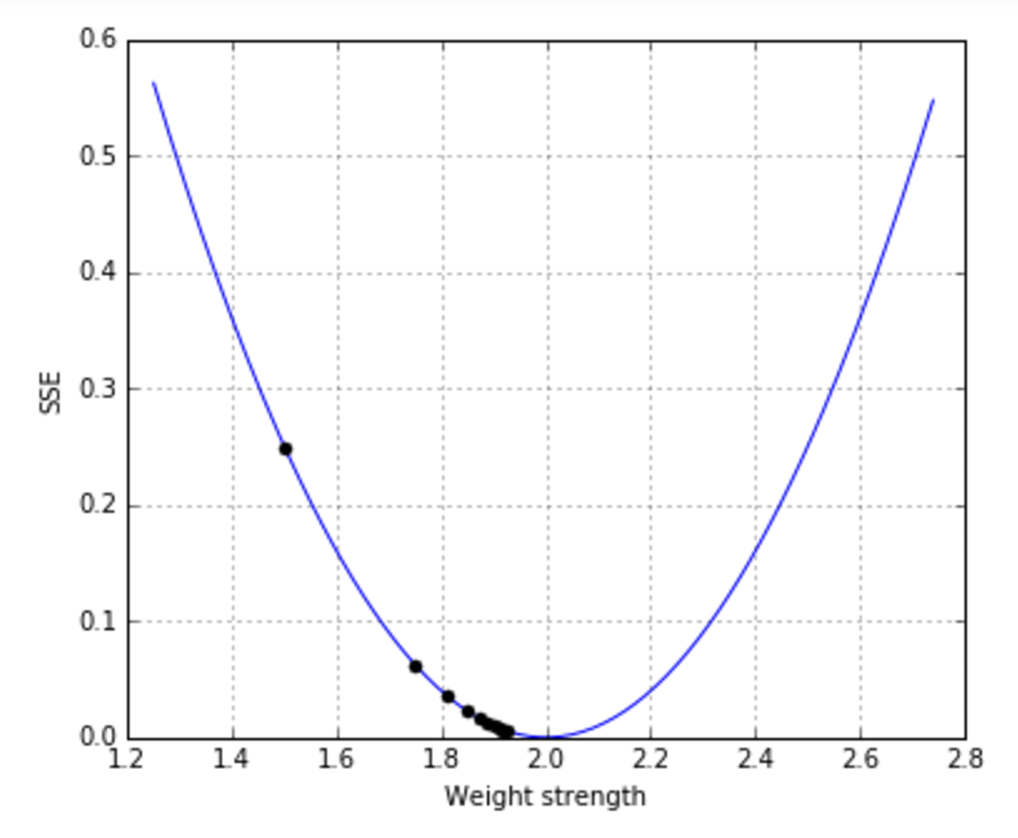
\includegraphics[width=0.5\textwidth]{images/error_lms.png}
\caption[Jeff Yoshimi.]{Gradient descent on the error surface for the LMS example discussed in Section. \ref{lms_example}. As the LMS rule is applied the weight strength changes in a way that minimizes sum squared error.}
\label{error_lms}
\end{figure}

(3) Applying the formula above
\begin{eqnarray*}
\Delta w_{i,j}  =  \epsilon a_i (t_j - a_j)
\end{eqnarray*}
we get
\begin{eqnarray*}
\Delta w_{1,2}  =  .5 \cdot 1 \cdot (2- 1.5) = .25
\end{eqnarray*}
We then use $\Delta w$ to update the weight value from its old value of 1.5, so that
\begin{eqnarray*}
w_{1,2}' = w_{1,2} + \Delta w_{1,2}  = 1.5 +.25  = 1.75
\end{eqnarray*}
So our new weight value is 1.75. 

(4) With this new weight, the network produces an output  $a_2' = 1 \cdot 1.75 = 1.75$. 

(5) The squared error is now $(2-1.75)^2=.25^2=.0625$, whereas before it was $.25$. So we have moved to the point $(1.75,.0625)$ in the graph  of the error surface in Fig. \ref{error_lms}. An improvement!  We have moved lower on the error curve; we have descended the error gradient.

In subsequent time steps we get:

\begin{eqnarray*}
w_{1,2}'' = 1.75 + .5 \cdot 1 \cdot (2 - 1.75) = 1.875 \\
w_{1,2}''' = 1.875 + .5 \cdot 1 \cdot (2 - 1.875) = 1. 9375 \\
\end{eqnarray*}
As you can see, applying this rule leads to SSE getting lower and lower, and the output getting closer and closer to the desired output of 2. Ten successive points on the error curve are shown in figure \ref{error_lms}.

\subsection{Practice Questions}

\newcounter{LMSCounter}

\noindent
\stepcounter{LMSCounter}
{\bf \theLMSCounter.}  Given $a_1 = 2 ,w_{1,2} = 2 ,t = 3 ,\epsilon = .25$, what are $a_2$, $SSE$, $w_{1,2}'$, $a_2'$, and SSE$'$? \\
{\bf Answer:}  \\
(1) $a_2 = a_1 \cdot w_{1,2} = 2 \cdot 2 = 4$ \\
(2) SSE = $(t-a_2)^2 = (3-4)^2 = (-1)^2 = 1$ \\
(3) $w_{1,2}' = w_{1,2} + \Delta w_{1,2}  = 2 +  \epsilon a_1 (t_2 - a_2) = 2 + (.25 \cdot 2 \cdot (3 - 4)) = 2+(-.5) = 1.5$\\
(4) $a_2' =  a_1 \cdot w_{1,2}' = 2 \cdot 1.5 = 3$ \\
(5) SSE$' = (3-3)^2 = 0$
\bigskip

\noindent
\stepcounter{LMSCounter}
{\bf \theLMSCounter.}  Given $a_1 = 2 ,w_{1,2} = 3, t = 5 ,\epsilon = .1$, what are $a_2$, $SSE$, $w_{1,2}'$, $a_2'$, and SSE$'$? \\
{\bf Answer:} \\
(1) $a_2 = 2 \cdot 3 = 6$ \\
(2) SSE $= (6-5)^2 = (-1)^2 = 1$ \\
(3) $w_{1,2}' = 3 + (.1 \cdot 2 \cdot (6-5)) = 3 + (-.2) = 2.8$ \\
(4) $a_2' = 2 \cdot 2.8= 5.6$ \\
(5) SSE$' = (5.6-5)^2 = .36$
\bigskip

\noindent
\stepcounter{LMSCounter}
{\bf \theLMSCounter.}  Given $a_1 = -1 ,w_{1,2} = 1, t = -2 ,\epsilon = .25$, what are $a_2$, $SSE$, $w_{1,2}'$, $a_2'$, and SSE$'$? \\
{\bf Answer:} \\
(1) $a_2 = -1$ \\
(2) SSE $= 1$ \\
(3) $w_{1,2}' = 1 + (.25 \cdot -1 \cdot (-2-(-1))) = 1 + .25 = 1.25$ \\
(4) $a_2' = -1.25$ \\
(5) SSE$' = (-2 - (-1.25))^2 = .56$
\bigskip

\noindent
\stepcounter{LMSCounter}
{\bf \theLMSCounter.}  Given $a_1 = 3 ,w_{1,2} = -.5, t = .8 ,\epsilon = .1$, what are $a_2$, $SSE$, $w_{1,2}'$, $a_2'$, and SSE$'$? \\
{\bf Answer:} \\
(1) $a_2 = -1.5$ \\
(2) SSE $= 5.29$ \\
(3) $w_{1,2}' = .69$ \\
(4) $a_2' = .57$ \\
(5) SSE$' = .053$
\bigskip

% Add some questions involving multiple inputs, and changing biases

\section{Linearly Separable and Inseparable Problems}
\label{linearlySeparable}

% glossary
% Add "donut" and other decision problem situations. Refer to sklearn page.

Two-layer feed-forward networks with linear output nodes, like LMS networks, are in a certain way limited. That limitation played  an important role in the history of neural networks, paving the way for studies of \emph{internal representations} in neural networks, which had lasting consequences both in machine learning and in connectionist applications of neural networks to psychology.  The limitation concerns the \glossary{linearly separable} classification tasks. Thus, in this section, and in much of the rest of the chapter, we focus on classification rather than regression.

% Do this with pictures for the classes, or even the inputs (see the wikipedia picture referenced above).
% Decision region and boundary should refer back to last chapter where there should be glossary entries
To understand what linear separability (and inseparability) are, recall that a classification task assigns each input to a different category. If we focus on networks with two input nodes and one output node, then we can plot a classification task as in figure \extref{visualize_classification} (Right), but we can also directly label the points as 0 and 1, as in figure \ref{F:decisionBoundaries}. When we create this type of plot, it often becomes immediately clear what the relationship between the categories is, in the input space. In figure \ref{F:decisionBoundaries} (Left), for example, we can immediately see that the two classes are distinct in the input space. Notice that we can separate the two categories by drawing a line between them, as in figure \ref{F:decisionBoundaries} (Middle). Such a line is, as we saw in section \extref{visClassification}, a \emph{decision boundary}, which has the effect of separating the input space in to two \emph{decision regions}, one for each possible classification. Input vectors in the region below the decision boundary will be classified as 0, while those in the region above the boundary will be classified as 1. However, note that for the task shown in figure \ref{F:decisionBoundaries} (Right) there is no way to use a line to separate the 0's and 1's perfectly.
% Use example? Each input vector will either be classified as in the class (1) or not in the class (0). For example, if the inputs were features of milk samples, then spoiled milk might produce an output of 0, good milk 1  

\begin{figure}[h]
\centering
\raisebox{-0.5\height}{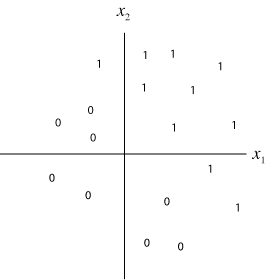
\includegraphics[scale=.4]{./images/decisionBoundaries1.png}}
\hspace*{.4in}
\raisebox{-0.5\height}{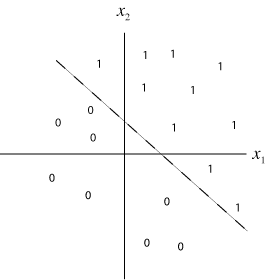
\includegraphics[scale=.4]{./images/decisionBoundaries2.png}}
\hspace*{.4in}
\raisebox{-0.5\height}{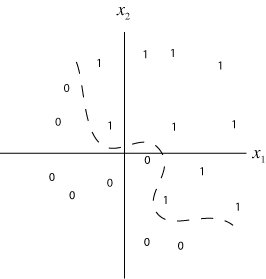
\includegraphics[scale=.4]{./images/decisionBoundaries3.png}}
\caption[Jeff Yoshimi.]{Three classification tasks. (Left) A linearly separable task. (Middle) A decision boundary that will solve the task. (Right) A linearly inseparable task and a non-linear decision boundary that can solve it.}
\label{F:decisionBoundaries}
\end{figure}
% Cohere this better with the section on tables and training tasks

If a classification task can be solved using a decision boundary which is a line (or, in more than 2-dimensions, a plane or hyperplane), the classification problem is called a \glossary{linearly separable} problem. Figure \ref{F:decisionBoundaries} (Middle) shows a linearly separable problem. When we cannot properly separate the categories with a line (or hyperplane), as in figure \ref{F:decisionBoundaries} (Right), the problem is \glossary{linearly inseparable}, there is no way to draw a line which separates the 0's and 1's in that example. There is no linear decision boundary for that problem (though there are non-linear decision boundaries that perfectly separate the classes, like the wavy curve shown in the figure).\footnote{First, note that in the case shown, we could still fit a line to the problem and we'd just have some error. Second, we will see that while LMS cannot solve this task, since it uses linear decision boundaries, other supervised classification algorithms like backprop exist that can solve these types of non-linearly separable classification task}

The goal of supervised learning of classification tasks is to set the weights of a network so that the decision boundary properly separates the two classes. The values of the weights and the output bias are like knobs that, when turned, will change where the decision boundary is: it can be rotated around and moved up and down. We want to turn the knobs so that they two  classes are properly separated.\footnote{Doing this amounts to minimizing error. When the decision boundary properly separates the two classes, SSE will be 0. If not, as in Fig. \ref{F:decisionBoundaries} (Right), there will be some error. What will SEE be in that case?}  However, LMS only allows linear decision boundaries. Other algorithms have more knobs, and can be used to create more complex decision boundaries and decision regions.
% Footnote on more complex decision regions here, or somewhere else? And the interesting material on how with more layers we get more complex regions. See the code comments at the end of this section. Also see the videos on this, which contain useful summary. References to Lipman and to Bishop chapter 4, e.g. figure 4. I feel I have written this up before so I may have it in notes.
  
Logic gates provide a convenient and historically important class of tasks that can be used to further illustrate these ideas. In appendix \extref{ch_logicgates} it is shown that logic gates can be represented as 2-1 feed-forward neural networks. Pairs of input nodes corresponding to statements P and Q connect to output nodes representing boolean combinations of truth values (0 for false, and 1 for true): P AND Q (true when both are true), P OR Q (true when at least one is true), and P XOR Q (true only when one is true). These can be depicted using the same kinds of classification plots as above (here using open dots for 0, and filled dots for 1). Fig. \ref{boolean_inputspace} shows the input space for the AND, OR and XOR logic gates. Note that AND and OR are linearly separable, and that XOR is not.

\begin{figure}[h]
\centering
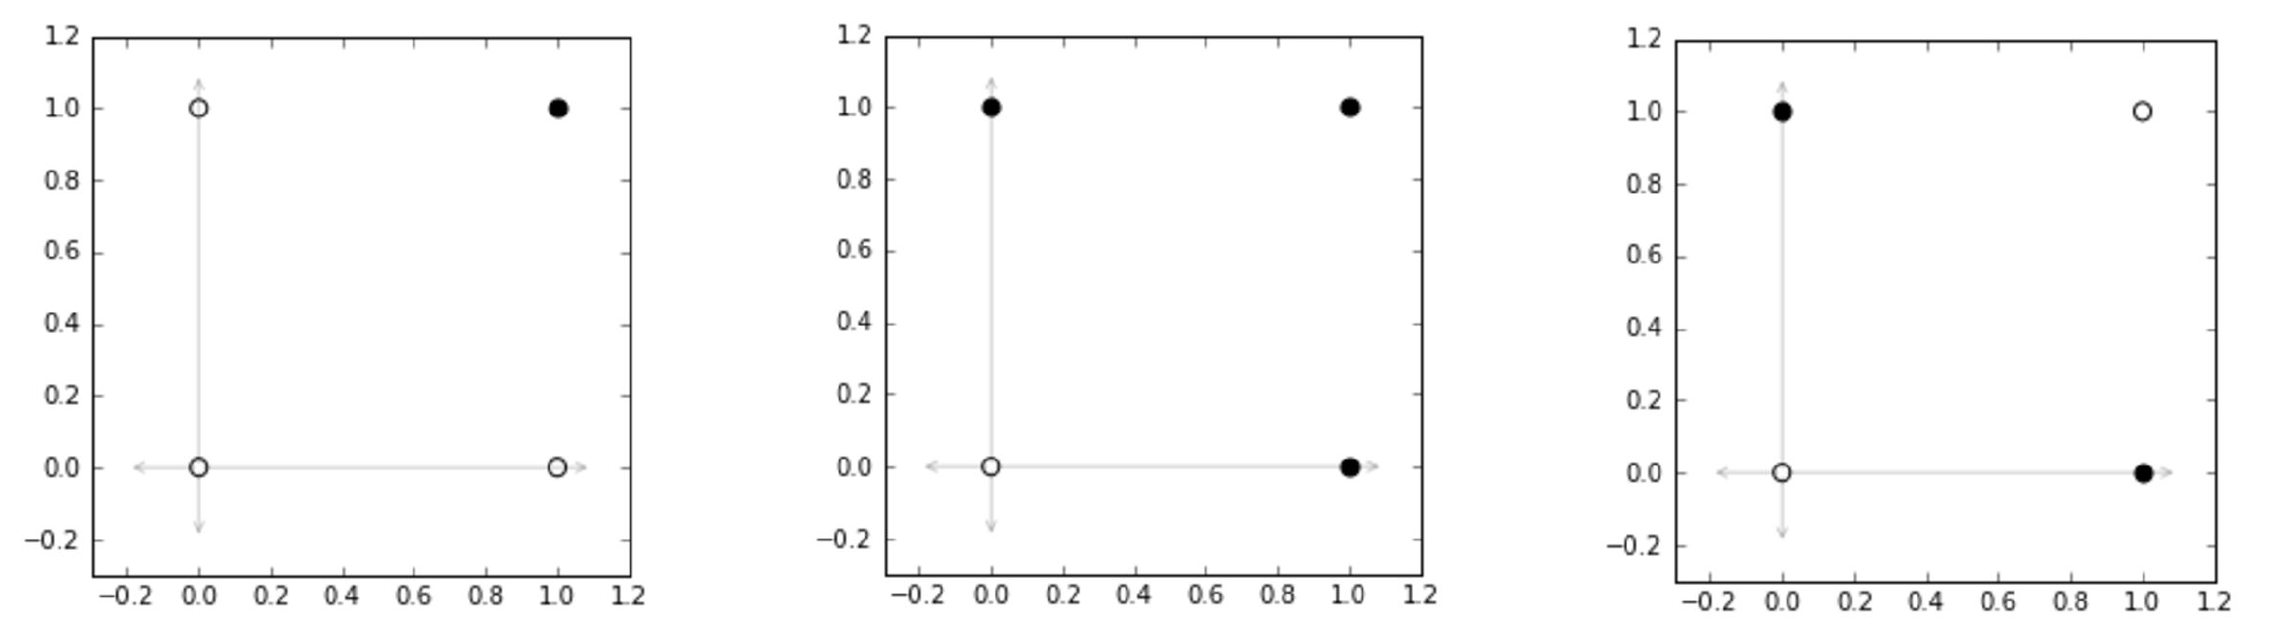
\includegraphics[width=0.9\textwidth]{images/booleanInputSpaces.png}
\caption[Jeff Yoshimi.]{Input spaces for AND (left), OR (middle), and XOR (right). Open dots correspond to 0, filled dots to 1. Which tasks are linearly separable?}
\label{boolean_inputspace}
\end{figure}

Now we get to the major problem affecting two layer networks trained using LMS: \emph{they cannot solve linearly inseparable classification tasks}, like XOR. That two-layer linear networks cannot solve these problems was a major issue in the early history of connectionism. In 1969 Marvin Minsky and Seymour Papert published a book called {\em Perceptrons} (perceptrons are a kind of 2-layer network trained by a variant of the LMS technique). In this book Minsky and Papert showed that such networks could not solve linearly inseparable problems \cite{minsky1969perceptrons}. This had a disastrous impact on neural network research in the following decade, during the ``dark ages'' of neural networks (see section \extref{dark_ages}). As Rumelhart and McClelland recall:

\begin{quote}
Minsky and Papert's analysis of the limitations of the one-layer perceptron\footnote{They are referring to a single weight layer connecting two layers of nodes. So what Rumelhart and McClelland call a ``one-layer'' network is what we have called a ``2-layer'' network}, coupled with some of the early successes of the symbolic processing approach in artificial intelligence, was enough to suggest to a large number of workers in the field that there was no future in perceptron-like computational devices for artificial intelligence and cognitive psychology (PDP 1, p. 112) \cite{rumelhart1986parallel}.
\end{quote}

However, as Rumelhart and McClelland go on to point out, these results don't apply to neural networks with more than 2 layers \cite{rumelhart1986parallel}. In fact, it has since been shown that multilayer neural networks with sigmoidal activation functions in the hidden layers are universal approximators in the sense that they can, in principle, approximate almost any vector-valued function (more specifically, any ``Borel measurable function from one finite-dimensional space to another'' \cite{hornik1989multilayer}.\footnote{This has since come to be known as the universal approximation theorem, and there is now a detailed Wikipedia page on the topic: \url{https://en.wikipedia.org/wiki/Universal_approximation_theorem}.}

So multi-layer feed-forward networks can solve linearly inseparable problems. Great!  But alas, there was another  problem. Initially there was no way to train multi-layered networks. LMS only works on 2 layer networks. Minsky and Papert, who first clearly identified this problem, recognized that adding hidden layers could surmount the limitations they described. However, they thought that multi-layer networks were {\em too} powerful, describing them as ``sufficiently unrestricted as to be vacuous'' (Rumelhart and McClelland, p. 112) \cite{rumelhart1986parallel}. In particular, Minsky and Papert pointed out that no one knew how such a network could be trained to solve specific pattern association tasks \cite{minsky1969perceptrons}.

Once algorithms were discovered that could be used to train multi-layer networks, it became possible to have networks learn solutions to linearly inseparable classification tasks (by finding non-linear decision boundaries) and to deal with much more complex problems than had previously been possible. The most famous algorithm of this type was backprop, which we turn to now.

\section{Backprop}

In this section we cover what was (at least until recently) the best known form of supervised learning: \glossary{backpropagation} ( or ``backprop''). Backpropagation is a powerful extension of the Least Mean Square  technique. As we saw, LMS only works for two-layer networks with linear activation functions. Backprop works for a much broader class of networks, in particular networks with non-linear (in particular, sigmoidal) activation functions and one or more hidden layers. As we will see, these hidden layers allow a network to transform inputs into different types of representation, and in doing so makes them quite powerful, and also psychologically interesting. 
%They do so by developing complex internal representations that map the input vectors (points in the input space) to hidden unit vectors (points in the hidden unit space). 

Backprop can be thought of as a generalization of the LMS technique or ``Delta rule'' described in Section \ref{lms_rule}. In fact backprop is sometimes called the ``generalized delta rule.'' This rule had been proposed as early as the late 1960s / early 1970s \cite{bryson1969applied, werbos1974beyond} and was independently discovered by several theorists in the 1980s \cite{le1986learning, parker1985learning}. It was popularized by Rumelhart, McClelland, and Williams in the late 1980s \cite{rumelhart1986parallel}. The discovery and popularization of backprop led to a revival of interest in neural networks in the 1980s and 1990s, following the ``dark ages'' of the 1970s (again, see chapter \extref{ch_history}).

\subsection{An Informal Account of the Algorithm}

% Put in some of the algorithm, either in a footnote or an appendix.
% The innovation was devising  a way to compute the derivative of the error function with respect to the hidden layer, or even multiple hidden layers.

We will not cover the details of the backpropagation algorithm in this chapter but will instead describe it in a qualitative way. As with LMS, the backprop algorithm conforms with the general template described in section \extref{SupervisedFirstPass}. Roughly:
\begin{enumerate}
\item Initialize the parameters of the network (which now includes hidden unit weights and biases) to random values.
\item Present an input vector from the training set.
\item Update the network.
\item Compute the error at each output node for this input vector (by comparing the actual output with the target output).
\item Use this error to update the weights and biases of the network, in a way that reduces the error function (e.g. SSE).
\end{enumerate}

The big innovation with backprop was figuring out how to do the last step on the hidden layer weights and biases, though we will not cover the details here.\footnote{Roughly speaking the output errors are ``back propagated'' to the hidden unit weights and biases. It is determined to what extent each hidden unit contributes to a given output nodes' error, ``blame is assigned,'' and on this basis the weights to the hidden layer are updated. This is where the term ``backpropagation'' comes from.}  

As with LMS, backprop works by minimizing an error function with respect to a training set, so that we have gradient descent on an error surface. However, since multi-layer feed-forward networks are more complex than 2-layer networks, the error surface is more complicated. With two-layer linear networks, the error surface has a relatively simple bowl-like structure, which often has a single minimum value at the low-point of a ``bowl'' shape. With a multi-layer non-linear network, the error surface can be more complex and wavy, and there can be multiple local minima (cf. figure \extref{local_minima}). These local minima can ``trap'' the gradient descent procedure, producing sub-optimal solutions.

One simple way to try to deal the issue is by re-initializing the parameters and re-running the algorithm. Each time this is done, the system moves to a different point on the error surface and tries finds the local minimum from that spot. By trying multiple times one can ``search'' for the lowest minimum possible.\footnote{Compare the way we searched for fixed points in chapter \extref{ch_dst}, by starting at different random points in state space.}  This is like dropping a marble at different spots on the error surface and comparing how low the marble goes each time. In this way we can find the lowest of several local minima (which might turn out to be the global minimum) and in this way we can try to improve a network's performance on a task. In practice, however, one uses advanced optimization techniques that do things to automatically search for a global minimum.\footnote{Currently the industry standard seems to be the ``Adam'' method: \url{https://arxiv.org/pdf/1412.6980.pdf}.}

\subsection{XOR and Internal Representations}

% Deep learning mention?  Ref. to cortex discussion?
We have not described in detail how the backprop algorithm works. However, we can get insight into what it does by considering what happens in the hidden layer of a network trained using backprop. In particular, we can begin to understand how multi-layer networks, like our brains, can solve problems by remapping input spaces to hidden unit spaces that contain useful internal representations. 

The classic example to illustrate these ideas is the XOR problem. Recall that XOR, considered as a vector valued function, is not linearly separable (figure \ref{boolean_inputspace}, right). Here is the labeled dataset we would use to train a network to implement XOR:
\begin{center}
\begin{tabular}{| c | c || c | }
\cline{1-3}
\multicolumn{2}{| c || }{inputs}
 & \multicolumn{1}{c|}{targets} \\
\hline
  $x_1$  & $x_2$ s& $t_1$  \\
\hline
  0 & 0 & 0  \\
\hline
 1 & 0 & 1  \\
\hline
 0 & 1 & 1 \\
\hline
1 & 1 & 0 \\
\hline
\end{tabular}
\end{center}
As we saw, two-layer networks with linear units cannot solve this type of problem, but a three-layer network with non-linear units can solve it. This is easy to confirm in Simbrain: try training an LMS and Backprop network on this data, and notice the difference in the minimum error you can achieve in the two cases. % Check and report these numbers?  
	
\begin{figure}[h]
\centering
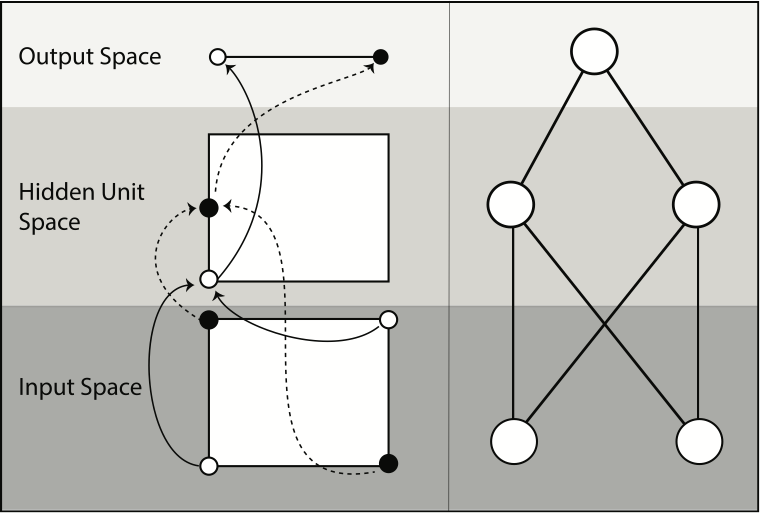
\includegraphics[width=0.7\textwidth]{images/xor_internal_rep.png}
\caption[Pamela Payne.]{A remapping of the input space to the hidden unit space in the XOR problem. Note that the bottom panel shows the input space for XOR, and that it is linearly inseparable. The network then maps $(0,0)$ and $(1,1)$,  to $(0,0)$ in the hidden unit space. $(0,1)$ and $(1,0)$ are mapped to $(0,.5)$ in the hidden unit space. Now notice that the hidden unit space is linearly separable!  Also notice that the hidden unit space has developed an internal representation of the two main cases of interest: just one unit is one (represented by $(0,.5)$) and both units are in the same state (represented by $(0,0)$). Thus the separated hidden unit states can be mapped to the appropriate output states.}
\label{xor_remapping}
\end{figure}


The key to backprop's superior performance is the way it \emph{re-maps} the linearly inseparable problem in the input space to a linearly separable problem in the hidden unit space, as shown in figure \ref{xor_remapping}. The crucial thing the hidden layer did was transform the input layer representation into a new internal representation, which includes a representation of ``only one unit is on'' and another representation of ``both units are in the same state.''  These two states are now linearly separable, and the output layer can easily separate them. The solution shown in the figure was produced by training a 2-2-1 network using backprop. Other solutions (corresponding to other minima in the error surface) can also be found. You are encouraged to try the experiment yourself in Simbrain. Train a backprop network on XOR, get it to a minimum on the error surface, and then check to see what hidden layer activations occur for each input.

\section{Internal Representations and Psychological Applications}\label{internalRepsFF}

% Work back in both chapter 1 themes: IAC (but  more for recurrent) and Triangle model. Definitely Spivey and JTrace  stuff with  continuous time-courses. See  Magnusson MTS talk. Quasi-regularity in language.
% Should this be it's own chapter?

We have seen that multilayer feed-forward networks trained by supervised learning methods (\eg backprop) will re-map the input space to reduce overall error on a learning task, for example by mapping linearly inseparable inputs to a separable set of points in the hidden units space. Even though these supervised learning methods are not generally taken to be neurally realistic\footnote{However, some circuits have been identified in the brain that may implement error-based supervised learning, \eg climbing fibers in the cerebellum (see chapter \extref{ch_neuro}). Error based learning that is similar in some ways to backprop is also emphasized in predictive coding accounts of the brain and predictive processing accounts of cognition.}, they are relevant to psychology and cognitive science, since neural networks trained using methods like backprop often develop internal representations that are similar to representations humans use.\footnote{That is, it is assumed that, even if backprop does not happen in most parts of the brain, it can still be used as a device to discover the kinds of representations that the brain finds. How the brain develops these representations is still a mystery, but backprop let's us at least see what those representations might look like and what function they might serve.}
% It's a bigger deal than that, they _outperform_ similar models in neuroscience

The idea that feed-forward networks trained by supervised learning methods learn to remap an input space and develop  psychologically realistic internal representations was the basis of much of the connectionists' work showing that neural networks could shed light on human perception and cognition. In this section, we focus on a few connectionist ideas that illustrate much of the work that came out of the first big wave of connectionism (the resurgence of interest in the 1980s and 1990s associated with the PDP group at UCSD). 

% Things to work on with EMPATH
% Clarify which part is backprop.  Not clear now in pics
% Does not follow nicely on xor the way nettalk does, in that the hidden layer reps are not as obviously psychologically relevant. Either improve description of them or change order.
% Relatedly, why do we care here about individual faces? In a way it's an artifact, isn't it?  In fact. since 14*6 = 84, it seems it might have just learned to distinguish happy, said, etc. for each person, then map from those to the output layer. I guess that's ok. But an individual face is not really an eigenface, so I'm missing something.
% Explain how this sets up  deep nets, which also both find features on their own (convolutional layers) and then compress via downsampling
% It is notable that the data is based on Ekman's famous work on facial expressions. Add that, at least in a footnote. Citation to POFA database (see Figure 1a) (Ekman & Friesen, 1976). \cite{ekman1976pictures} Note Ekman, also at UCSD, is a famous psychoogist who used this dataset used to argue for universality of basic emotions. "Through a series of studies, Ekman found a high agreement across members of diverse Western and Eastern literate cultures on selecting emotional labels that fit facial expressions. Expressions he found to be universal included those indicating wrath, grossness, fear, joy, loneliness, and shock", "This data set contains photos of 14 actors portraying expressions that are reliably classified as happy, sad, afraid, angry, surprised, or disgusted by naive observers"

An example is Gary Cottrell's  emotion recognition model, EMPATH, shown in figure \ref{face_net}.\footnote{See \url{http://authors.library.caltech.edu/6983/1/DAIjcn02.pdf} \cite{dailey2002empath}.} This network was trained using multiple images of multiple people, each of whom made different facial expressions. The network had several hidden layers, including a layer of edge detectors (outputs of Gabor filters), and a layer that used principle components analysis or PCA, which is similar to Oja's rule (see chapter \extref{ch_unsupervised}) to do a dimensionality reduction of the previous layer, pulling out the most significant features of that layer. The second-to-last node layer of the network was called a ``Gestalt layer''. It produced responses similar to face-detectors in the ventral stream of the human visual system  (see chapter \extref{ch_neuro}). The output layer has a one-hot encoding of six basic emotions \cite{dailey2002empath}. 

\begin{figure}[h]
\centering
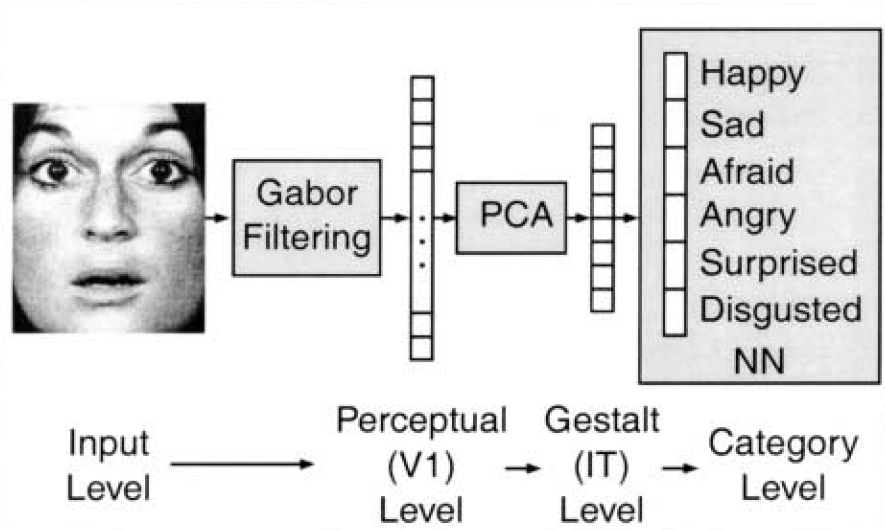
\includegraphics[width=0.5\textwidth]{images/face_network.png}
\caption[From Adolphs, Cottrell, Dailey and Padgett, 2002  \cite{dailey2002empath}.]{Structure of Cottrell's EMPATH emotion recognition network. On the left is a grid of nodes that respond directly to an image. This layer contains over 40,000 nodes. The image inputs are then processed using a layer of weights (``Gabor filtering'') that produce responses in the ``perceptual level'' nodes similar to responses of edge detector neurons in the visual cortex. Another layer of weights performs PCA to reduce the perceptual level to a ``gestalt'' layer of 50 nodes, that produces responses similar to responses in the ventral steam of the human visual system. The final layer of 6 nodes does the actual classification into different emotion categories, using least mean squares. }
\label{face_net}
\end{figure}

Cottrell focused particularly on the second-to-last ``Gestalt'' layer of the network, which  developed nodes that are responsive to particular faces. Cottrell has said that the face recognition nodes in his network act a lot like face recognition neurons in the brain.\footnote{\url{http://tdlc.ucsd.edu/events/boot_camp_2015/Cottrell_Backprop-representations.pdf}.}  Like real face-recognition neurons in the ventral stream of cortex (more specifically in area IT), these neurons respond to a picture of someone even if their eyes were occluded, and respond less strongly the more a face image is rotated. The network produced these representations of people \emph{even though it was never told about individuals}. It was only trained to recognize emotions. It did this entirely on its own, as an artifact of the training process \cite{dailey2002empath}. 

% Finding optimal stimulator for an internal node using gradient descent (in a new way).
One thing you can do with this kind of network is visualize the internal representations it develops. If you focus on one of the face recognition nodes, and then find what visual input it is most tuned to, a ``ghostly looking face'' can be observed (see figure \ref{holon}). This image is a kind of visualization of the network's internal template or representation for a particular person \cite{dailey2002empath}. It might be similar to what gets activated in dreams and imagination.\footnote{For a more recent example that takes this idea much further, see \url{https://research.googleblog.com/2015/06/inceptionism-going-deeper-into-neural.html} \cite{mordvintsev2015inceptionism}. Also see \url{https://distill.pub/2017/feature-visualization/}.}
% https://en.wikipedia.org/wiki/Eigenface
% Need proper citation for distill article
% The resulting low-dimensional object-level representation is specific to the facial expression and identity variations in its input, as is the population of so-called face cells in the inferior temporal cortex
% any face in training set a linear combination of eigenfaces. 
% especially clear in https://www.cs.ucsb.edu/~mturk/Papers/jcn.pdf

\begin{figure}[h]
\centering
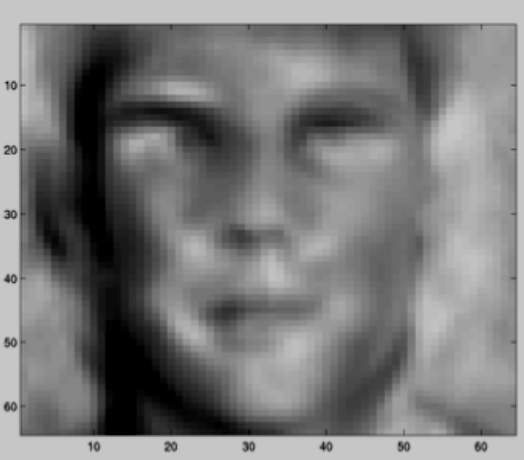
\includegraphics[width=0.3\textwidth]{images/holon.png}
\caption[From \url{http://cseweb.ucsd.edu/\~gary/258a/Backprop.pdf}.]{Optimal input pattern for a hidden (``Gestalt'') layer face node. Shows what kinds of inputs the unit will respond to.}
\label{holon}
\end{figure}

% A model of phonetics
Another case where a feed-forward network trained using backprop finds psychologically interesting internal representations is NETtalk, a model of reading English words aloud, created by Terrence Sejnowski and Charles Rosenberg in 1987 \cite{sejnowski1987parallel}. It is one of the most famous early examples of a connectionist network, that is, a neural network used to shed light on human psychology, in this case the structure of language processing.

The network is a three layer feed-forward network with the structure shown in figure \ref{net_talk}.  The network was trained to speak aloud. It was presented with written letters in English and was trained to pronounce those letters. The input layer codes for a moving window of letters, one of which is taken to be the current input and the rest of which provide the network with information about neighboring letters.\footnote{Each letter is coded by a 29-dimensional vector (involving one-hot, one-of-29 representations of particular letters, with three additional nodes representing punctuation and word boundaries). The letters surrounding a letter in a word (3 before and 3 after) are coded to provide context which can be used to  correctly pronounce a letter. Thus there were $29 \times 7 = 203$ input units. This kind of moving window is a way of approximating temporal processes in a static feed-forward network.} The output layer contains 26 units encoding different features of phonemes (components of spoken letters), including voicing and vowel height. The hidden layer has 80 hidden units \cite{sejnowski1987parallel}. 

\begin{figure}[h]
\centering
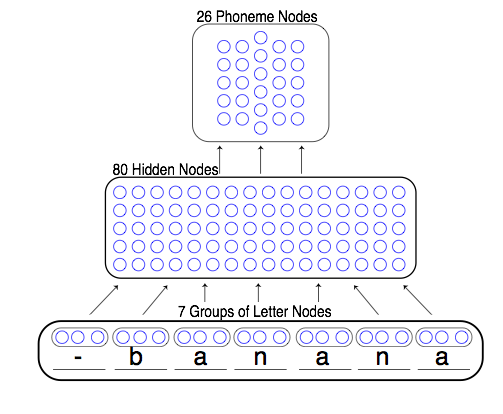
\includegraphics[width=0.5\textwidth]{images/net_talk.png}
\caption[Pamela Payne.]{NETtalk models converting written words to sounds, \ie reading aloud. Each letter group has 27 nodes (not the 3 shown). When trained using backprop, it developed internal representations of vowels and consonants, without having been told about them.}
\label{net_talk}
\end{figure}
% This needs pictures of the vowel vs. consonant part of its state space. That dimension of the discussion is being left out.
% Definitely redo and somehow convey the 27 nodes per group. Maybe just draw them out?  Or use ellipses

There are about 18,000 weights and biases in the network, so that the error surface is 18,000 dimensional! Backprop was used to train these weights and biases to solve the problem. The network was trained on a corpus of 1000 common words. It took several days to get the error to a reasonable level using their circa 1987 computer \cite{sejnowski1987parallel}. A slightly modified version of the network could generalize from these 1000 training samples to pronouncing 90 percent of the 20,000 words in a standard English dictionary correctly. The network was shown to perform well with noisy input and to gracefully degrade \cite{sejnowski1987parallel}. So it did quite well.
%This was not like XOR in Simbrain where in a few seconds the network was trained. Training took a long time (and training still does take a long time, days or even weeks or more, in industrial settings, even with huge computers). 

There are two things that made this example striking. First, the network again developed psychologically plausible internal representations, which it was not programmed to do. For example, the hidden units learned to produce a complete separation of consonants and vowels. Vowels produced hidden unit vectors in one region of hidden unit space, while consonants produced hidden unit vectors in another region of hidden unit space. The network was not told about the difference between vowels and consonants--it simply learned these categories while it was trained on the pronunciation task \cite{sejnowski1987parallel}. This showed  how in learning a mapping from sensory inputs to motor outputs, psychologically meaningful categories could take form in a network's hidden unit space.

Second, the sounds the networks produced could be artificially synthesized and played back. This was done at several stages in training. Initially the network produced a babble of sounds, like a baby. But as it came to learn the task is got better and better, until it produced somewhat fluent speech \cite{sejnowski1987parallel}. This made it quite palpable what was going on: the network was slowly getting better, in a way that sounded vaguely like a child learning to read. I encourage you to listen to the (somewhat creepy) process: \url{https://www.youtube.com/watch?v=gakJlr3GecE}. So again, even if backprop is not neurally plausible, it seems to be doing something \emph{like} what the brain does, and it does so by developing psychologically realistic representations of vowels and constants.\footnote{There are many other studies of learned representations and their psychological realism, in many  domains of cognitive science and neuroscience. A book length  study of semantic cognition, for example, is \cite{rogers2004semantic}.}
% Expand on the semantic cognition book with a few more paragraphs. It's got very simple and  compelling examples. Maybe also add the development book out of UCSD. 

% In another example, due to Hinton, backprop was used to train a network to describe relationships between members of two families, one American and one Italian. The network could be asked a question like ``who was Sophia's sister". The network developed hidden layer nodes that  represented whether a given person was Italian or American, and whether a person was first-generation, second-generation, etc. Using this information the network could draw inferences. What is interesting is that it developed these representations of nationality and generation without being told to \cite{hinton1986learning}.
